
\subsection*{Experimental setup}
\begin{figure}[ht]
	\centering
	\includegraphics{figures/experimentalSetup.png}
	\caption{Illustration of the photoluminescence spectroscopy setup. The excitation light follows the path highlighted in blue to induce PL on the sample. The pathway of the PL signal is highlighted in red.}
	\label{fig:experimentalSetup}
\end{figure}

\autoref{fig:experimentalSetup} illustrates our experimental setup for PL spectroscopy measurements.
The blue path highlights the incident beam which excites the sample and induces photoluminescence.
Our laser generates light with a central wavelength of \SI{402}{nm} which passes through an excitation filter to select light with a wavelength of \SI{405}{nm}.
A dichroic mirror directs the light to lens 1 which focusses incident light on the sample's surface.
The path that is taken by the emitted photoluminescence light is highlighted in red.
Starting from the sample's surface, this light is collected and collimated by lens 1 and passes through the dichroic mirror.
To ensure that the excitation light is completely removed from the emission path, we use a longpass filter with a cut-on wavelength of \SI{420}{nm}.
Finally, lens 2 focusses the light onto an optical fibre which directs the light to our spectrometer (LR2, Lasertack GmbH).

Both the laser and the spectrometer are controlled with a microcontroller which in turn is connected to a pc.
This arrangement makes it possible to control the laser power, exposure time and the time between sample excitation and signal acquisition.
The latter is set to \SI{500}{ms}.

\subsection*{Samples and measurement parameters}

\begin{table}[ht]
	\centering
	\begin{tabular}{|p{3.5cm}|p{2.5cm}|p{6cm}|}
		\hline
		Sample Category & No. of Samples & Sample Type\\
		\hline
		Non-plastic & 12 &
		\begin{itemize}[noitemsep,topsep=0pt]
			\item Sand
			\item Wood
			\item Posidonia Oceanica (Plant)
			\item Sepia Officinalis (Bone)
			\item Echinocardium Cordatum (Shell)
			\item Hexaplex Eggs (Shell)
			\item Monodonta Turbinata (Shell)
			\item Neverita Josephina (Shell)
			\item Lithophyllum Racemus
		\end{itemize}\\
		\hline
		Plastic (manufacturer) & 26 &
		\begin{itemize}[noitemsep,topsep=0pt]
			\item Polyamide (PA)
			\item Polycarbonate (PC)
			\item Polyethylene (PE)
			\item Low-density polyethylene (LDPE)
			\item High-density polyethylene (HDPE)
			\item Polyethylene terephthalate (PET)
			\item Polymethylmethacrylate (PMMA)
			\item Polypropylene (PP)
			\item Polystyrene (PS)
			\item Polyvinyl chloride (PVC)
		\end{itemize}\\
		\hline
		Plastic (retail) & 8 &
		\begin{itemize}[noitemsep,topsep=0pt]
			\item LDPE
			\item HDPE
			\item PET
			\item PP
		\end{itemize}\\
		\hline
	\end{tabular}
	\caption{Overview of samples used for this study.}
	\label{tab:samples}
\end{table}

\begin{table}[ht]
	\centering
	\begin{tabular}{|p{3.5cm}*{4}{|c}|}
		\hline
		Sample Category & \multicolumn{2}{c|}{Measurement 1} & \multicolumn{2}{c|}{Measurement 2}\\
		\cline{2-5}
		{} & $\mathrm{P_{laser}}$ [mW] & $\mathrm{t_{ex}}$ [ms] & $\mathrm{P_{laser}}$ [mW] & $\mathrm{t_{ex}}$ [ms]\\
		\hline
		Non-plastic & 0.5\textendash130 & 300 & 0.2\textendash2.8 & 300\\
		\hline
		Plastic (manufacturer) & 5\textendash130 & 300 & 0.5\textendash100 & 300\\
		\hline
		Plastic (retail) & 0.5\textendash130 & 300\textendash1500 & 0.5\textendash104 & 300\\
		\hline
	\end{tabular}
	\caption{Summary of samples and measurement parameters. For each sample, two measurements were taken where the laser power ($\mathrm{P_{laser}}$), the exposure time ($\mathrm{t_{ex}}$) and alignments in the setup were changed.}
	\label{tab:measParameters}
\end{table}

Our PL spectra dataset is generated from 46 samples which consists of non-plastic materials from the riverine and marine environment and plastics from different manufacturers and retail products.
A summary of the dataset is presented in \autoref{tab:samples}.

For each sample, we take two different measurements, where we change the laser power $\mathrm{P_{laser}}$, the exposure time $\mathrm{t_{ex}}$ and alignments in the setup.
These adjustments are made to acquire a signal with a low background noise.
A list of these measurement parameters is presented in \autoref{tab:measParameters}.
All our spectra are measured in the range 295 \textendash 1000 nm.
